\documentclass[conference]{IEEEtran}
%Template version as of 6/27/2024

\usepackage{cite}
\usepackage{amsmath,amssymb,amsfonts}
\usepackage{algorithmic}
\usepackage{graphicx}
\usepackage{textcomp}
\usepackage{xcolor}
\usepackage{url}
\def\BibTeX{{\rm B\kern-.05em{\sc i\kern-.025em b}\kern-.08em
    T\kern-.1667em\lower.7ex\hbox{E}\kern-.125emX}}

\makeatletter
\def\abstract{\normalfont
    \@IEEEabskeysecsize\bfseries\textit{\abstractname}:\ \relax
    \@IEEEgobbleleadPARNLSP}
\def\IEEEkeywords{\normalfont
    \@IEEEabskeysecsize\bfseries\textit{\IEEEkeywordsname}:\ \relax
    \@IEEEgobbleleadPARNLSP}
\makeatother

\begin{document}

\title{Survival and Recovery of Learned and Model Predictive Locomotion Controllers in MuJoCo}

\author{\IEEEauthorblockN{Manvendra Vikram Singh}
\IEEEauthorblockA{\textit{VIT Bhopal University}\\
Bhopal, India \\
manvendra.25bai10188@vitbhopal.ac.in}
\and
\IEEEauthorblockN{Maddala Jashwanth}
\IEEEauthorblockA{\textit{VIT Bhopal University}\\
Bhopal, India \\
maddala.25bai10796@vitbhopal.ac.in}
\and
\IEEEauthorblockN{Khushi Roy}
\IEEEauthorblockA{\textit{VIT Bhopal University}\\
Bhopal, India \\
khushi.25bai11506@vitbhopal.ac.in}
\and
\IEEEauthorblockN{Sehajdeep Singh}
\IEEEauthorblockA{\textit{VIT Bhopal University}\\
Bhopal, India \\
sehajdeep.25bai10096@vitbhopal.ac.in}
\and
\IEEEauthorblockN{Paridhi Rathi}
\IEEEauthorblockA{\textit{VIT Bhopal University}\\
Bhopal, India \\
paridhi.25bai11559@vitbhopal.ac.in}
\and
\IEEEauthorblockN{Dhanya Thakur}
\IEEEauthorblockA{\textit{VIT Bhopal University}\\
Bhopal, India \\
dhanya.25bai11347@vitbhopal.ac.in}
}

\maketitle

\begin{abstract}
Comparing locomotion controllers requires more than checking whether a robot stays upright after a push. The disturbance profile, collision model, and recovery rule can change the interpretation of a result. This paper presents an independent simulation comparison of learned and model predictive controllers for the Unitree Go1 quadruped. Three policies trained with proximal policy optimization and one predictive-sampling controller are evaluated in a shared full-collision MuJoCo model. The study contains 92 trials: 20 nominal trials, 36 rectangular-pulse trials, and 36 triangular-pulse trials. A gait-aware policy with a calf-clearance penalty completed all five nominal trials, while the predictive controller completed two. Under rectangular pushes, the final learned policy completed none of 18 trials and the predictive controller completed six. With triangular pushes at the same peak forces and durations, these counts became six and twelve. However, only five learned-policy trials and four predictive-controller trials met the stricter tracking and recovery conditions. The triangular pulses commanded half the rectangular impulse, so the difference cannot be attributed to waveform alone. The results distinguish physical survival from successful recovery and show why force profiles and failure rules must be reported explicitly. They describe the tested controllers and conditions, not an exact reproduction of the motivating benchmark or a general ranking of control methods.
\end{abstract}

\begin{IEEEkeywords}
legged locomotion, model predictive control, proximal policy optimization, MuJoCo, disturbance rejection, reproducible evaluation
\end{IEEEkeywords}

%======================================================================
\section{Introduction}

A quadruped can remain standing after a push and still fail its locomotion task. It may move too slowly, drift sideways, or fail to return to the commanded velocity. These outcomes are different from a fall, but a survival-only score does not distinguish them. Similarly, two pushes with the same peak force can deliver different impulses when their force profiles differ. Both choices matter when interpreting a controller comparison.

Akki and Chen compared model predictive control (MPC) and reinforcement learning (RL) for Unitree Go1 locomotion in MuJoCo, considering disturbance rejection, energy use, and terrain conditions \cite{akki2025}. Their study motivates the present work. Rather than claiming to recover the exact controller implementations, we build an independent comparison with explicit controller settings, saved policies, common measurement rules, and retained failure trajectories.

The learned controllers are neural policies trained with proximal policy optimization (PPO). The MPC controller uses the upstream MuJoCo MPC (MJPC) predictive-sampling planner with a Go1 task written for this study. All reported evaluations use the same native MuJoCo plant. A fixed forward-velocity command keeps the task simple enough to examine how controller behavior changes under lateral disturbances.

The study addresses three questions. First, which selected controllers complete nominal walking when full body collisions are checked? Second, how do physical completion and tracking recovery differ under rectangular and triangular pushes? Third, what do the recorded mechanical work and decision times indicate about the cost of the tested behavior?

Our contribution is a transparent empirical evaluation, not a new control algorithm. It consists of a common native evaluation path, a 92-trial dataset with frozen controller identities, and a comparison that separates survival, tracking qualification, and recovery. Failed trials remain part of the results. The triangular experiment is a separately labeled follow-up, chosen after inspecting the rectangular results, rather than a replacement for them.

%======================================================================
\section{Background and Scope}

\subsection{Learned and Predictive Control}

MuJoCo provides articulated-body simulation with contact, which makes it suitable for examining legged control in a common physical model \cite{todorov2012}. PPO learns a policy by collecting interactions and optimizing a clipped surrogate objective \cite{schulman2017}. MuJoCo Playground provides robot-learning environments built on the accelerated MuJoCo XLA (MJX) backend \cite{zakka2025}, and we train with its Brax PPO implementation \cite{freeman2021}. We use the Playground Go1 task as the starting point for the learned policies, with a fixed command and study-specific gait terms.

MJPC provides simulation-based predictive control. Its predictive-sampling method perturbs a nominal control spline, rolls out the candidates in MuJoCo, and retains the lowest-cost plan \cite{howell2022}. Our native bridge calls that upstream planner. The additional work in this study is the Go1 task, the controller interface, and the common evaluation and analysis code. We do not present the sampling algorithm as a new method.

\subsection{Relationship to the Motivating Benchmark}

Table~\ref{tab:scope} identifies the main differences from the published benchmark \cite{akki2025}. Its simulation settings are listed in Table~2 of that paper. Its fixed-magnitude perturbation tests apply 150~N for 0.2~s at the center of mass along the positive and negative $x$-axis and the negative $y$-axis. The force profile of these tests is not stated in the text, but the released perturbation data show a constant 150~N force over the 0.2~s window \cite{akkirepo}. Its maximum-disturbance search instead uses a triangular pulse of 0.2~s, increased in 10~N steps until failure. Our initial push experiment used rectangular pulses; the follow-up used symmetric triangles. Both studies classify body--ground contact as failure regardless of later recovery, and both compute cost of transport from positive joint work.

\begin{table}[htbp]
\caption{Scope of the Independent Reconstruction Compared with the Motivating Study}
\begin{center}
\footnotesize
\begin{tabular}{|p{1.75cm}|p{2.75cm}|p{2.75cm}|}
\hline
\textbf{Item} & \textbf{Published benchmark \cite{akki2025}} & \textbf{Present study} \\
\hline
Robot, command & Go1, 0.5~m/s forward & Go1, 0.5~m/s forward \\
\hline
Robot mass & 12~kg (declared) & 12.743448~kg (compiled model) \\
\hline
Physics step & 1~ms & 4~ms \\
\hline
Floor friction & 0.6, 0.3, 0.3 & 0.6, 0.005, 0.0001 \\
\hline
Trial duration & 50~s & 30~s nominal; 12~s push \\
\hline
PPO & RL Baselines3 Zoo \cite{rlzoo}, Optuna-tuned, $10^6$ steps & Brax and MuJoCo Playground, fixed settings, about $2.2\times10^8$ steps \\
\hline
MPC task & Four residual groups & Thirteen task terms \\
\hline
Fixed pushes & 150~N, 0.2~s; $+x$, $-x$, $-y$ & 50/100/150~N, 0.2~s; $\pm y$ \\
\hline
Pulse shape & Constant (fixed tests); triangular (maximum search) & Rectangular; triangular follow-up \\
\hline
Terrain & Flat, slippery, uneven & Flat only \\
\hline
\end{tabular}
\label{tab:scope}
\end{center}
\end{table}

These differences prevent a direct numerical reproduction claim. We do not use our outcomes to confirm or refute the original paper's force limits or energy values. The comparison concerns the selected policies and the declared MJPC task in our own evaluation contract.

%======================================================================
\section{Controller Implementation}

\subsection{Shared Robot and Actuation}

The evaluation model has a floating base and twelve actuated joints. Its state contains 19 generalized position coordinates and 18 generalized velocity coordinates. Both controller types produce joint-position targets, held over each 20~ms control interval. Each joint $j$ is driven by a proportional position actuator with gain $K_p=35$~N\,m/rad, whose output is saturated at the model's force limit $\bar\tau_j$:
\begin{equation}
\tau_j^{\mathrm{act}}(t)=\operatorname{sat}_{\bar\tau_j}\!\bigl(K_p\bigl(q_j^{\mathrm{des}}(t)-q_j(t)\bigr)\bigr).
\label{eq:actuator}
\end{equation}
Here, $q_j$ is the joint angle and $\operatorname{sat}_{\bar\tau}(x)=\min(\max(x,-\bar\tau),\bar\tau)$. The limits are 23.7~N\,m for the first two joints of each leg and 35.55~N\,m for the third. Following the pinned Playground task, the derivative gain $K_d=0.5$~N\,m\,s/rad is implemented as passive joint damping $-K_d\dot q_j$, together with the model's joint friction loss. These passive terms are therefore not bounded by $\bar\tau_j$ and are not part of the actuator work measured in Section~\ref{sec:work}.

Physics advances every 4~ms. The compiled model retains the Newton solver and its one-iteration setting from the pinned task. The floor friction vector is 0.6, 0.005, and 0.0001 for sliding, torsional, and rolling friction. The full collision geometry and home pose are identical across evaluated controllers.

\subsection{PPO Policies}

We evaluate three saved policies: \emph{PPO reference}, \emph{PPO gait}, and \emph{PPO gait + calf}. The reference uses the fixed-command Playground task without the added walking schedule. The gait policy adds phase observations and rewards for a four-beat walking pattern. The final policy also penalizes inadequate calf clearance.

The actor receives body-frame linear velocity, gyroscope readings, projected gravity, joint angles relative to the home pose, joint velocities, the previous action, and the command. This gives 48 inputs for the reference and 50 for the gait policies, which add the sine and cosine of gait phase. A separate privileged observation feeds the critic during training; it is not an actor input during evaluation. Both networks have hidden layers of 512, 256, and 128 units with SiLU activation.

The policy action $\mathbf a_t$ sets a target relative to the home configuration:
\begin{equation}
\mathbf q_t^{\mathrm{des}}=\mathbf q^{\mathrm{home}}+0.5\,\mathbf a_t,
\label{eq:action}
\end{equation}
where the scale is in radians. Evaluation restores the saved network and observation normalizer, uses deterministic inference, and disables observation noise. The adapter preserves the pinned task's action-history update order: the previous action exposed to the next observation is two control decisions behind, as during training.

All three policies were trained from random initialization with training seed zero. The saved configuration uses a learning rate of $3\times10^{-4}$, discount factor 0.97, entropy coefficient 0.01, 128 parallel environments, 20-step unrolls, 32 minibatches of size 256, and four updates per batch. Training episodes contain 1,000 control steps, or 20~s. Training was requested for 200 million environment steps; Table~\ref{tab:policies} reports the step counts of the saved checkpoints used here, which exceed that request and differ between variants.

\begin{table}[htbp]
\caption{Saved Learned Controllers Used in Evaluation}
\begin{center}
\footnotesize
\begin{tabular}{|p{1.45cm}|c|p{2.6cm}|r|}
\hline
\textbf{Policy} & \textbf{Inputs} & \textbf{Added reward terms} & \textbf{Steps} \\
\hline
PPO reference & 48 & None beyond the fixed-command task & 217,907,200 \\
\hline
PPO gait & 50 & Contact schedule, swing height, support penalties & 217,907,200 \\
\hline
PPO gait + calf & 50 & Gait terms and calf-clearance penalty & 229,376,000 \\
\hline
\multicolumn{4}{l}{One training run per variant, seed 0.}
\end{tabular}
\label{tab:policies}
\end{center}
\end{table}

Training uses the feet-only collision model for MJX throughput, with observation-noise level 1.0 and no random push perturbations. Testing transfers the saved actors to the native full-collision model. This distinction is important: avoiding body contact is checked physically during evaluation, but the training collision model does not provide the same body--ground contact response.

The walking schedule has period 0.8~s, swing fraction 0.22, swing order rear-left, front-left, rear-right, front-right, and target swing height 0.08~m. The added reward weights are 2.0 for contact agreement, 1.0 for swing height, $-1.5$ for extra swing feet, and $-2.0$ for having no supporting foot. The final policy adds weight $-2.0$ to
\begin{equation}
r_{\mathrm{calf}}(t)=\sum_{i=1}^{4}\max\!\left(\frac{m_c-h_i(t)}{m_c},0\right),\qquad m_c=0.015~\mathrm{m},
\label{eq:calf}
\end{equation}
where $h_i(t)$ is the lowest point of the modeled calf capsule of leg $i$ above the floor. In the feet-only training model, it is estimated from calf-body transforms and the full-model capsule endpoints. This is a clearance surrogate, not physical full-collision training. The original Playground reward components and scales remain recorded in the training manifests. The three policies have different reward definitions and unequal training steps, so they are selected controller variants, not a controlled reward ablation.

\subsection{MJPC Controller}

The MJPC controller uses the upstream sampling planner at revision \texttt{ff572a2} \cite{mjpc}. At each control decision, the bridge supplies exact position, velocity, and simulation time. It runs four optimization iterations and requests the current action from the resulting plan. This is an information advantage over the PPO actor, whose inputs are limited to its observation.

Candidate trajectories cover 0.24~s and are parameterized by three linearly interpolated spline points. Each iteration rolls out 128 trajectories, including the current nominal plan, using four planner threads. The exploration fraction is 0.03, scaled for each actuator by half its control-range width; it is not a fixed 0.03~rad noise standard deviation. The task settings were selected on development trials with initial-state seeds 0, 1, and 2, then frozen before the main evaluation.

The planner solves
\begin{equation}
\begin{aligned}
&\min_{\boldsymbol\theta}\ \sum_{k=0}^{H-1}\ell(\mathbf x_k,\mathbf u_k),\qquad
\mathbf x_{k+1}=f_{\mathrm{MuJoCo}}(\mathbf x_k,\mathbf u_k),\\
&\ell(\mathbf x,\mathbf u)=\sum_{i=1}^{13}\frac{w_i}{2}\left\|\mathbf r_i(\mathbf x,\mathbf u)\right\|_2^2,
\end{aligned}
\label{eq:mpc}
\end{equation}
where $\boldsymbol\theta$ are the spline parameters, $\mathbf x_k$ is the predicted state, $\mathbf u_k$ is the position command, and $H$ is the discrete planning horizon. The residual groups contain 58 scalar entries in total, and Table~\ref{tab:mjpc} gives their weights. The task includes a 0.278~m torso-height target, the same walking schedule and 15~mm calf-clearance target as the final PPO task, and a one-second ramp for the foot-height and stride references. The forward-velocity target remains 0.5~m/s from the start.

\begin{table}[htbp]
\caption{Fixed MJPC Task Terms and Weights}
\begin{center}
\footnotesize
\begin{tabular}{|l|r|p{3.9cm}|}
\hline
\textbf{Term} & \textbf{Weight} & \textbf{Quantity penalized} \\
\hline
Height & 500 & Torso-height error \\
Velocity & 60 & Body-frame planar velocity error \\
Upright & 100 & Torso tilt \\
Heading & 5 & Departure from world forward heading \\
Effort & 0.03 & Actuator force relative to its limit \\
Posture & 2 & Departure from the home joint pose \\
Gait & 300 & Foot-height error against the walking reference \\
Calf clearance & 5,000 & Calf-clearance shortfall \\
Balance & 100 & Capture-point proxy relative to mean foot position \\
Angular velocity & 0.5 & Base angular velocity \\
Foot placement & 100 & Body-frame foot-position reference error \\
Support force & 300 & Swing-foot load or stance-foot load deficit \\
Nonfoot collision & 100 & Nonfoot contact proximity or penetration \\
\hline
\end{tabular}
\label{tab:mjpc}
\end{center}
\end{table}

These residuals are explicit task priors. They do not generate joint commands directly and are not the motivating paper's residual implementation. The upstream sampler remains unseeded; initial-state seeds do not seed its exploration.

%======================================================================
\section{Experimental Protocol and Measurements}

\subsection{Nominal and Push Trials}

The main dataset contains five nominal trials per controller, giving 20 trials with a requested horizon of 30~s. Joint angles at reset receive independent Gaussian perturbations with standard deviation 0.01~rad. Seeds 100 through 104 identify the five initial poses. Each controller starts from the same pose for a given seed, and these seeds were not used in MJPC development.

The final PPO policy and MJPC also receive lateral pushes at peak forces of 50, 100, and 150~N. Both world-frame directions, positive and negative $Y$, are tested at initial-state seeds 100, 101, and 102. Each push starts at 5~s, lasts 0.2~s, and occurs in a 12~s trial. The rectangular experiment has 36 trials. The triangular follow-up repeats this grid for another 36 trials without retraining or changing planner settings. Nominal trials are not repeated because they contain no pulse. The total is therefore 92 evaluated trials, excluding training and development rollouts.

For pulse start $t_0$, duration $D$, peak $F_p$, and unit world direction $\mathbf d$, the force is
\begin{equation}
\begin{aligned}
&\mathbf F(t)=F_p\,\mathbf d\,g\!\left(\frac{t-t_0}{D}\right),\qquad 0\leq \frac{t-t_0}{D}<1,\\
&g_{\mathrm{rect}}(s)=1,\qquad g_{\mathrm{tri}}(s)=1-|2s-1|,
\end{aligned}
\label{eq:pulse}
\end{equation}
and is zero outside the pulse interval. Its intended scalar impulse is
\begin{equation}
J_{\mathrm{rect}}=F_pD,\qquad J_{\mathrm{tri}}=\tfrac{1}{2}F_pD.
\label{eq:impulse}
\end{equation}
Thus, the rectangular grid commands 10, 20, and 30~N\,s, while the triangular grid commands 5, 10, and 15~N\,s. The force is applied through the trunk body's external-force field at its center of mass, with no separately imposed torque. The force is evaluated at the midpoint of each 4~ms physics step and held over that step, and the delivered impulse is integrated from those values. With this sampling, the largest applied triangular value is $0.98F_p$, while the delivered impulse of a full pulse equals \eqref{eq:impulse} exactly. A trial that fails before or during a pulse may receive less than the intended impulse.

All pushes have a fixed onset. Since the gait period is fixed, these tests cover only one scheduled onset phase, not a distribution of gait phases. The directions are world-lateral rather than guaranteed body-lateral because heading can drift.

\subsection{Physical Failure, Tracking, and Recovery}

Every physics step checks for penetrating nonfoot--floor contact, an inverted torso, a nonfinite state, or a MuJoCo warning, and each control decision checks for a controller error. A trial stops immediately at its first failure. Calf or thigh contact is sufficient to fail; the rule does not require a complete body fall. This conservative rule is shared by every controller. All stopped trajectories remain in the dataset.

Let $\mathbf v_{xy}^{b}(t)$ be the measured body-frame planar velocity and $\mathbf v^*=[0.5,\ 0]^{\top}$~m/s the command. Define
\begin{equation}
\begin{aligned}
e(t)&=\bigl\|\mathbf v_{xy}^{b}(t)-\mathbf v^*\bigr\|_2,\\
\mathrm{RMSE}(\mathcal W)&=\sqrt{\frac{1}{|\mathcal W|}\sum_{t_k\in\mathcal W}e(t_k)^2},
\end{aligned}
\label{eq:rmse}
\end{equation}
where $\mathcal W$ contains the recorded control-rate samples in the selected window. A nominal pass requires 30~s without failure, finite data, positive net forward displacement, and RMSE of at most 0.15~m/s after a two-second warmup.

For push trials, \emph{physical completion} means finishing the 12~s horizon without the physical or numerical failure conditions. \emph{Strict success} additionally requires prepush RMSE of at most 0.15~m/s over 2 to 5~s and demonstrated recovery. Recovery is the first postpulse time at which the tracking error remains within tolerance for a full 0.5~s:
\begin{equation}
\begin{aligned}
t_{\mathrm{rec}}=\min_{t\geq t_e}\bigl\{t-t_e:\ &e(\tau)\leq 0.15~\mathrm{m/s}\\
&\forall\,\tau\in[t,\,t+0.5~\mathrm{s}]\bigr\},
\end{aligned}
\label{eq:recovery}
\end{equation}
with $t_e=t_0+D$ and $\tau$ ranging over recorded samples. The record must cover the entire dwell interval, and failure at any later point still prevents strict success. The dwell test is evaluated at the 50~Hz control-recording rate, whereas physical failures are checked at 250~Hz. A recovery time is undefined when no qualifying interval exists; it is not replaced by the trial duration. Failure before the push is reported separately and cannot establish a disturbance limit.

\subsection{Gait, Mechanical Work, and Timing}\label{sec:work}

Gait measurements use instantaneous penetrating foot--floor contacts in the common native model. We report agreement with the prescribed contact schedule, the fraction of samples with exactly one swing foot, and the fraction with all feet airborne. A swing foot is a foot without recorded ground contact. These are descriptive contact measures, not a guarantee of a natural or dynamically optimal walk.

For actuator torque $\tau^{\mathrm{act}}_{j,k}$ from \eqref{eq:actuator} and joint velocity $\dot q_{j,k}$ at physics sample $k$, robot mass $m$, gravity $g$, and positive net world-forward displacement $\Delta x$, positive mechanical work and cost of transport are
\begin{equation}
\begin{aligned}
E_+&=\Delta t\sum_k\sum_{j=1}^{12}\max\bigl(\tau^{\mathrm{act}}_{j,k}\,\dot q_{j,k},\,0\bigr),\\
\mathrm{CoT}_+&=\frac{E_+}{mg\Delta x}.
\end{aligned}
\label{eq:cot}
\end{equation}
The declared integration step is $\Delta t=4$~ms. A separate 20~ms endpoint estimate is retained to examine sampling sensitivity. This metric is positive actuator mechanical work, not battery energy, and follows the positive-work form used in \cite{akki2025}. Work and net displacement cover the full recorded trial, including startup. Speed, tracking, and gait summaries exclude the first two seconds. Aggregate nominal metrics use completed trials only; failed runs receive no invented steady-state values. Nonpositive displacement gives an undefined cost of transport.

Decision timing measures observation and host handling plus blocking PPO inference or MJPC planning. PPO compilation is excluded. The main dataset is collected serially on a CPU. Triangular trials use two worker processes pinned to disjoint sets of six logical CPUs, while each MJPC instance retains four planner threads. Their timing includes resource contention and is not combined with the serial latency comparison.

Both controllers execute synchronously offline. Physics does not advance while an action is being computed, and a late action is not inserted into a delay model. Consequently, these experiments do not test real-time control under missed deadlines.

\subsection{Statistics and Verification}

We retain counts by force, direction, and controller, with Wilson 95\% intervals \cite{wilson1927} in the outcome figures. There are only three initial-condition trials per push cell and five per nominal controller. The intervals describe these small observed samples; they do not establish training-seed generalization or a statistically reliable overall ranking. Counts pooled over the disturbance grid are descriptive totals across different conditions, not repeated trials of one common success probability.

Verification checks planned-trial coverage, saved summaries, model and checkpoint identities, matched initial poses, physics timestamps, integrated work, force vectors, and delivered impulse. Tracking qualification, dwell-based recovery, and strict success were independently recalculated from the saved trajectories. All 18 final-policy triangular trajectories also matched the corresponding rectangular trajectories exactly through the first five seconds, before the push. This supports the PPO backend comparison without asserting deterministic equivalence for unseeded MJPC planning.

%======================================================================
\section{Results}

\subsection{Nominal Locomotion}

Fig.~\ref{fig:survival} shows physical survival over the nominal horizon. PPO reference failed in all five trials at approximately 0.512~s. PPO gait also failed in all five, between 0.380 and 0.384~s. In both groups, the recorded failure geometry was the front-left calf capsule. These are failures under the full-collision contact rule, not evidence that the policies never produced forward motion in their feet-only training environments.

\begin{figure}[htbp]
\centerline{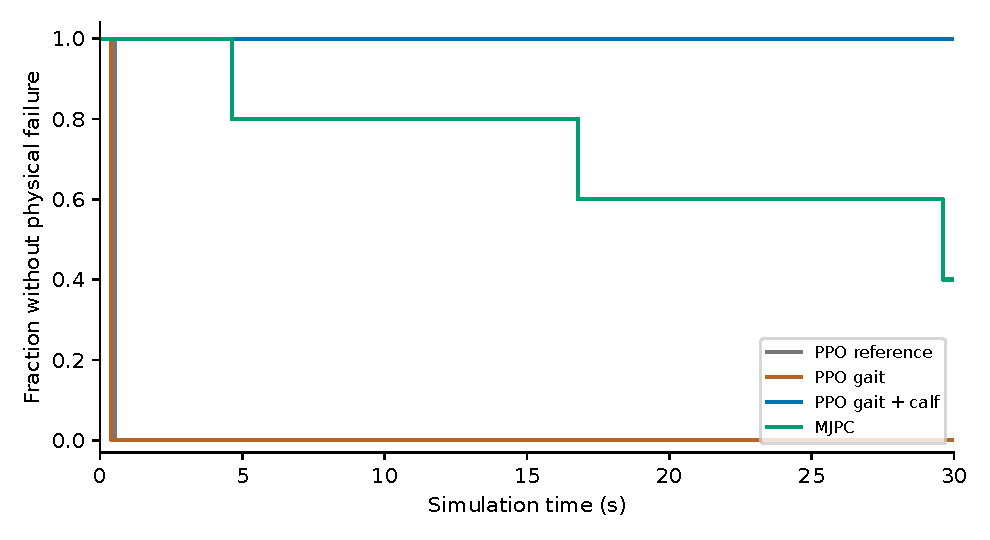
\includegraphics[width=\columnwidth]{figures/nominal-survival.pdf}}
\caption{Fraction of nominal trials remaining without physical failure. Each controller has five trials. Curves end at the requested 30~s horizon; the final calf-clearance PPO completes all five and MJPC completes two.}
\label{fig:survival}
\end{figure}

Table~\ref{tab:nominal} summarizes the completed trials. PPO gait + calf passed all five nominal tests. MJPC passed two, with its other trials stopping at 4.604, 16.788, and 29.584~s after calf--floor contact. The selected final PPO therefore completed nominal walking more consistently in this sample. This result alone does not establish that the clearance reward caused the improvement.

\begin{table}[htbp]
\caption{Nominal Outcomes and Survivor-Only Mean Metrics}
\begin{center}
\footnotesize
\begin{tabular}{|l|c|c|c|c|c|}
\hline
\textbf{Controller} & \textbf{Passes} & \textbf{$n$} & \textbf{Speed} & \textbf{RMSE} & \textbf{CoT$_+$} \\
 & & & \textbf{(m/s)} & \textbf{(m/s)} & \\
\hline
PPO reference & 0/5 & 0 & -- & -- & -- \\
PPO gait & 0/5 & 0 & -- & -- & -- \\
PPO gait + calf & 5/5 & 5 & 0.4218 & 0.1013 & 1.3333 \\
MJPC & 2/5 & 2 & 0.3935 & 0.1404 & 1.4881 \\
\hline
\multicolumn{6}{p{7.6cm}}{$n$: completed trials contributing metrics. Speed is mean forward body velocity; RMSE is planar body-frame error \eqref{eq:rmse}. Both exclude the 2~s warmup.}
\end{tabular}
\label{tab:nominal}
\end{center}
\end{table}

Survivor counts differ, so Table~\ref{tab:nominal} is not an unbiased controller-wide energy ranking. Sample standard deviations of speed, RMSE, and CoT are 0.0005, 0.0003, and 0.0015 for the final PPO, and 0.0063, 0.0042, and 0.0314 for MJPC. The small PPO variation reflects a deterministic policy and narrowly perturbed initial poses, not broad robustness.

Fig.~\ref{fig:contacts} shows the recorded contact sequence for initial seed 100. Across completed nominal trials, the final PPO's mean phase agreement was 0.9587 and its exactly-one-swing fraction was 0.9251. The corresponding MJPC survivor means were 0.8795 and 0.6824. All-feet-airborne fractions were 0.0090 and 0.0025. Schedule agreement is measured against the study's specified four-beat pattern; it is not a universal gait-quality score.

\begin{figure}[htbp]
\centerline{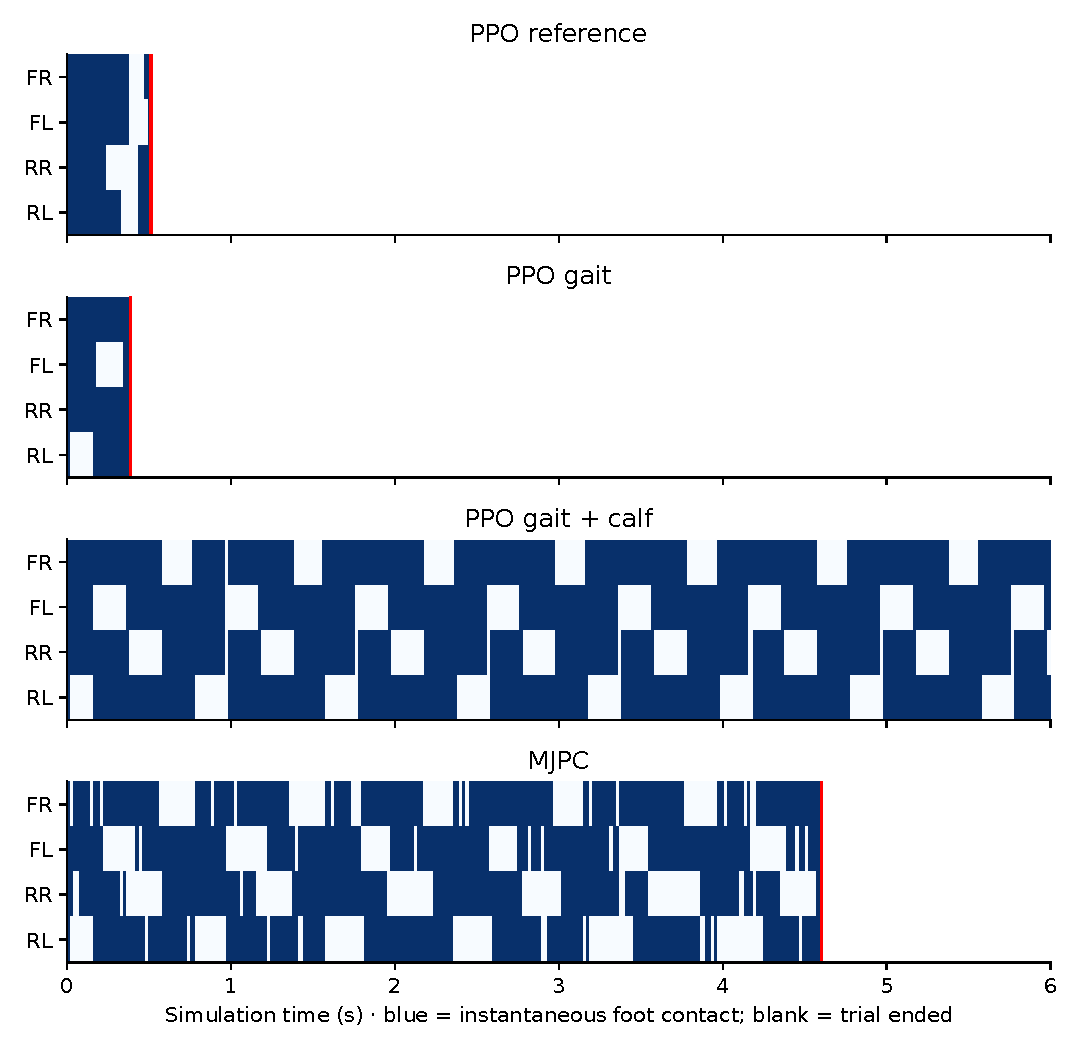
\includegraphics[width=\columnwidth]{figures/foot-contact-rasters.pdf}}
\caption{Foot-contact records for the first 6~s of nominal initial seed 100. Dark blue indicates penetrating foot--floor contact, light segments within a record indicate no contact, and blank space after the red stop marker indicates an ended trial. FR, FL, RR, and RL denote front-right, front-left, rear-right, and rear-left. The MJPC trial shown is not one of its two completed nominal trials.}
\label{fig:contacts}
\end{figure}

Passing the body-frame velocity rule did not guarantee a straight path. Fig.~\ref{fig:paths} illustrates lateral drift at initial seed 100, where the final PPO ended approximately 1.40~m to the side after 30~s. Across its five completed trials, the final PPO's lateral displacement ranged from 1.26 to 1.44~m toward negative $Y$, with a mean final heading of $-8.62^\circ$. The two completed MJPC trials drifted further, ending 4.91 and 5.11~m toward positive $Y$ with a mean final heading of $22.86^\circ$; they do not appear in Fig.~\ref{fig:paths} because the MJPC trial at seed 100 failed at 4.60~s. World-frame planar RMSE was 0.1154~m/s for the final PPO and 0.2517~m/s for MJPC survivors. These measurements limit any claim of accurate straight-line walking for either controller.

\begin{figure}[htbp]
\centerline{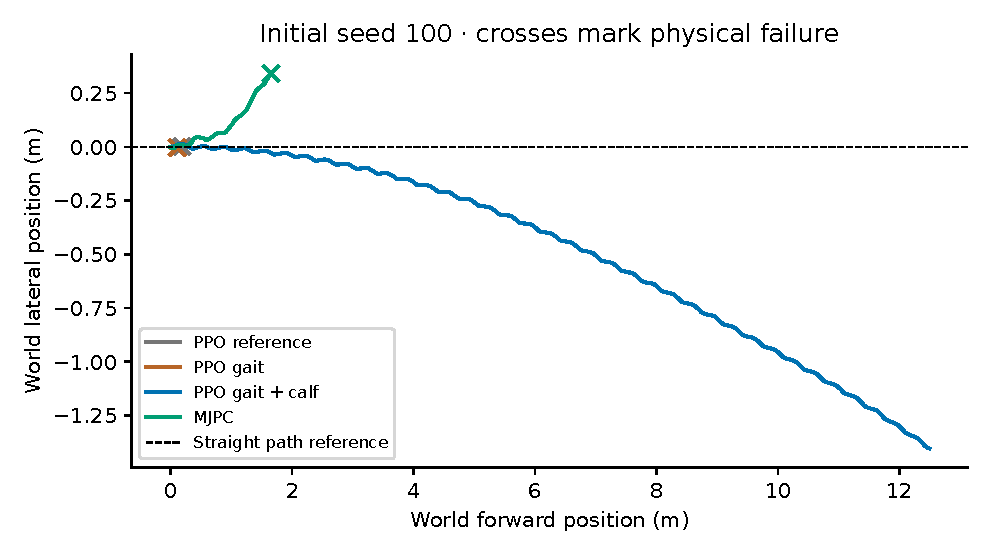
\includegraphics[width=\columnwidth]{figures/nominal-paths.pdf}}
\caption{Recorded world-frame paths at initial seed 100. Crosses mark physical failures. The final PPO's completed path drifts from the straight-line reference. Unequal trace lengths are retained rather than extrapolated.}
\label{fig:paths}
\end{figure}

\subsection{Physical Survival and Recovery Under Pushes}

Table~\ref{tab:push} reports descriptive totals over the 18 push trials for each controller and pulse shape. No final-PPO rectangular trial completed. MJPC completed six rectangular trials, but only two met strict success, recovering in 1.88 and 2.72~s. Under triangular pulses, the final PPO completed six trials and achieved strict success in five. MJPC completed twelve and achieved strict success in four.

\begin{table}[htbp]
\caption{Push Outcomes Pooled over the Force--Direction Grid}
\begin{center}
\footnotesize
\begin{tabular}{|l|l|c|c|c|c|}
\hline
\textbf{Controller} & \textbf{Pulse} & \textbf{Compl.} & \textbf{Strict} & \textbf{Prepush} & \textbf{Full} \\
 & & & \textbf{succ.} & \textbf{qual.} & \textbf{pulse} \\
\hline
PPO gait + calf & Rect. & 0 & 0 & 18 & 18 \\
PPO gait + calf & Tri. & 6 & 5 & 18 & 18 \\
MJPC & Rect. & 6 & 2 & 14 & 13 \\
MJPC & Tri. & 12 & 4 & 13 & 16 \\
\hline
\multicolumn{6}{p{7.2cm}}{Each row has 18 trials: three peak forces, two directions, and three initial poses.}
\end{tabular}
\label{tab:push}
\end{center}
\end{table}

The distinction between completion and success is substantial. Eight of twelve completed MJPC triangular trials did not meet the strict criterion. A completed trial may have excessive prepush tracking error or may never demonstrate the required sustained recovery. For example, one completed 150~N negative-$Y$ MJPC trial had a recorded recovery interval but failed prepush qualification. It therefore remains a strict failure.

\begin{figure*}[t]
\centerline{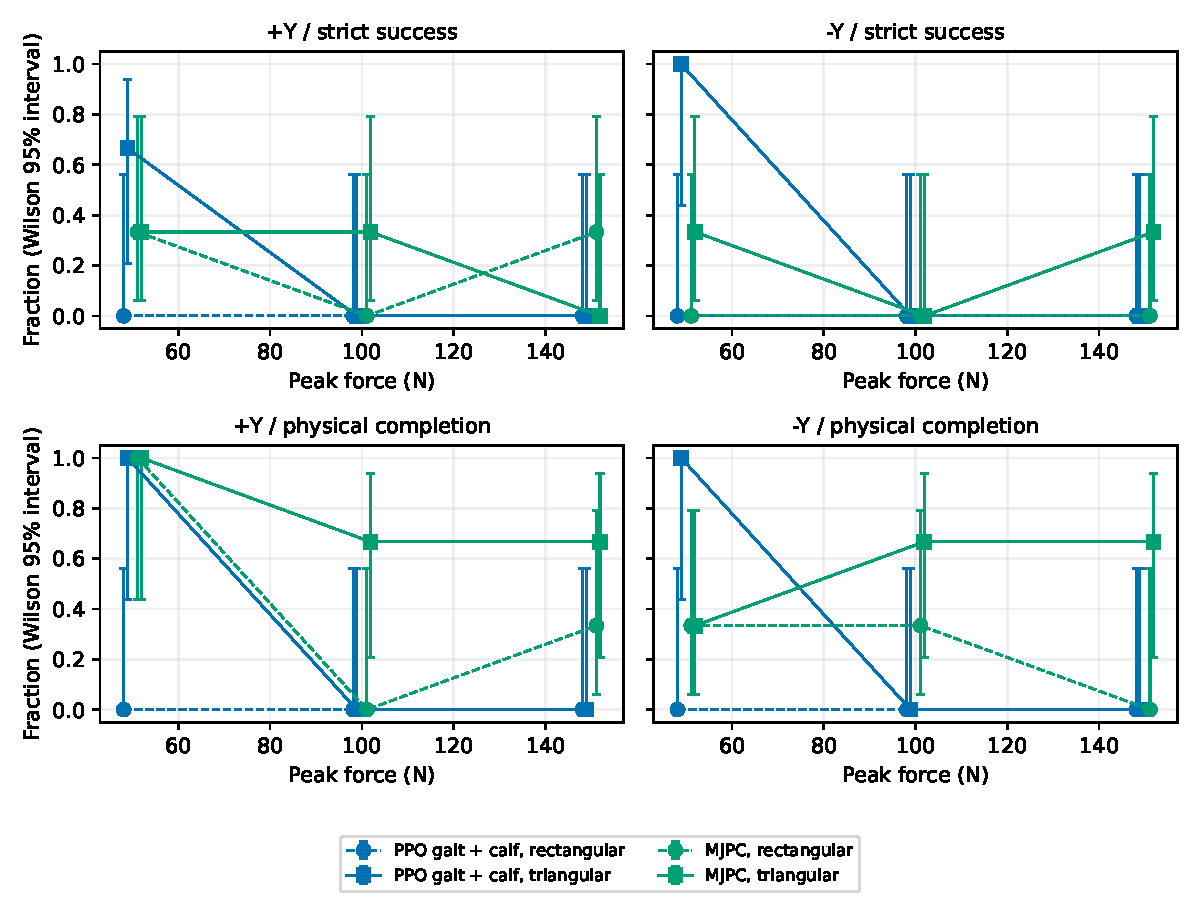
\includegraphics[width=0.82\textwidth]{figures/push-outcomes-by-peak.pdf}}
\caption{Strict success and physical completion versus peak force, separated by world push direction. Each point has three trials with a Wilson 95\% interval. Small horizontal offsets separate overlapping markers and do not denote additional force levels. Connecting lines aid reading and are not fitted robustness curves.}
\label{fig:peak}
\end{figure*}

Fig.~\ref{fig:peak} retains both direction-specific outcomes and confidence intervals. All six final-PPO 50~N triangular trials completed. Strict success was two of three in positive $Y$ and three of three in negative $Y$. The remaining completed positive-$Y$ trial never demonstrated the required 0.5~s recovery dwell. Successful final-PPO recovery times ranged from 0.68 to 2.20~s after the pulse end.

At 100 and 150~N, the final PPO completed no triangular trials. Its twelve failures comprised nine nonfoot contacts and three torso inversions. In contrast, MJPC completed four of six triangular trials at each peak force when directions were pooled. Strict MJPC successes were two at 50~N, one at 100~N, and one at 150~N, with recovery times from 1.14 to 2.28~s. These sparse, nonmonotonic counts do not identify a maximum robust force.

Several MJPC trials did not receive the complete commanded disturbance. In the triangular grid, the trial at the scheduled 100~N positive-$Y$ condition failed at 4.004~s before receiving any push, and the 150~N positive-$Y$ trial at seed 100 failed at 5.184~s after receiving approximately 14.808 of the intended 15~N\,s. In the rectangular grid, the 150~N negative-$Y$ trial at seed 101 failed at 1.868~s before its push, and four trials failed during the pulse after receiving 18.8 to 27.6~N\,s of the intended 20 or 30~N\,s. All are retained in Table~\ref{tab:push}, and none can be treated as a complete-pulse disturbance-tolerance observation.

\subsection{Peak Force and Impulse}

The lower-force PPO outcome changes when the pulse becomes triangular, but \eqref{eq:impulse} shows why calling this a waveform-only benefit would be misleading. At 50~N and 0.2~s, the triangle commands 5~N\,s instead of 10~N\,s, while the controller and its training are unchanged.

\begin{figure*}[t]
\centerline{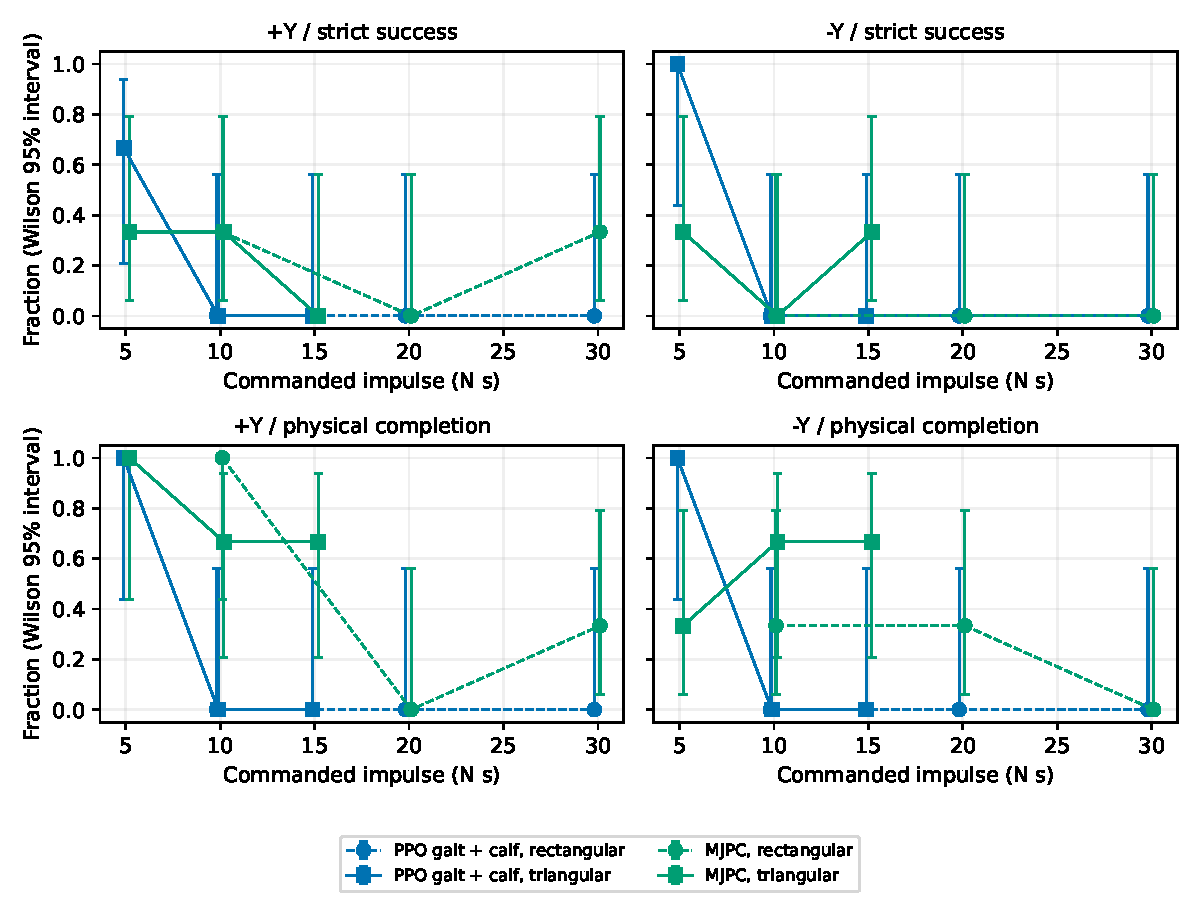
\includegraphics[width=0.82\textwidth]{figures/push-outcomes-by-impulse.pdf}}
\caption{The outcome counts from Fig.~\ref{fig:peak} plotted against commanded impulse. Equal horizontal coordinates can represent different peak forces and pulse profiles. Some failed MJPC trials received less than the commanded impulse; the delivery counts in Table~\ref{tab:push} identify this distinction.}
\label{fig:impulse}
\end{figure*}

Fig.~\ref{fig:impulse} shows the same outcomes against commanded impulse. The final PPO fails all six 100~N triangular trials at 10~N\,s, just as it fails all six 50~N rectangular trials at 10~N\,s. This is a useful equal-impulse comparison within the existing grid, but the peak forces and temporal profiles still differ. It does not establish impulse as the sole cause or define a transferable threshold. Overall, the tested policy handles the mildest triangular condition, while its tolerance remains limited at the other tested conditions.

\subsection{Mechanical Work and Decision Time}

The survivor-only positive-work CoT means are 1.3333 for the final PPO and 1.4881 for MJPC. The 50~Hz endpoint estimates are 1.1299 and 1.2961, respectively, approximately 15.3\% and 12.9\% below the declared 250~Hz estimates. This sampling dependence matters when comparing energy numbers. The higher-rate measurement is our declared quadrature, not a demonstrated continuous-time ground truth.

Fig.~\ref{fig:latency} presents serial nominal decision times on the local AMD Ryzen~5 4600HS CPU. For completed nominal trials, the final PPO mean was 0.665~ms and the MJPC mean was 242.7~ms. Across all five MJPC nominal trials, trial-mean times ranged from approximately 216 to 244~ms. Every recorded nominal MJPC decision exceeded the 20~ms control interval.

\begin{figure}[htbp]
\centerline{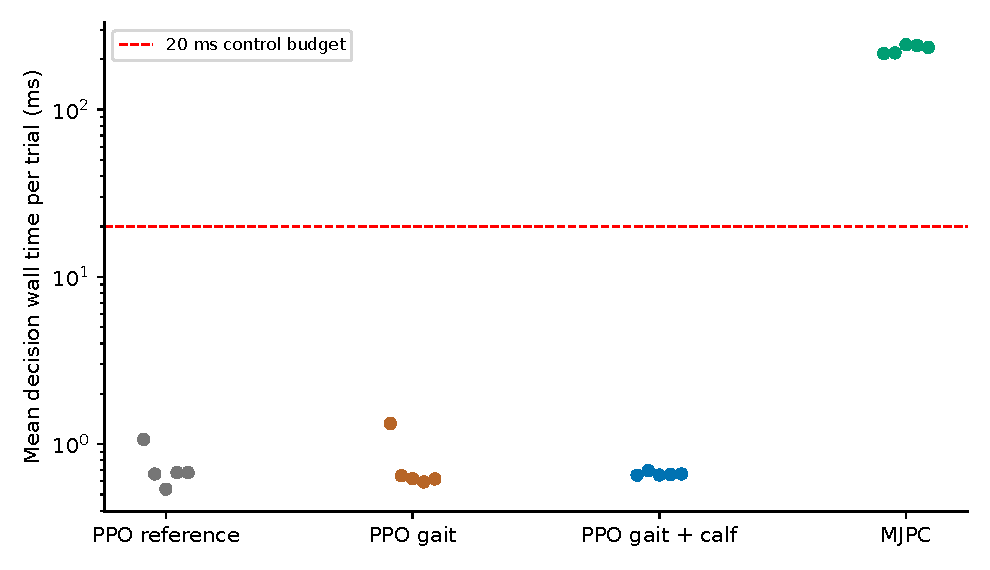
\includegraphics[width=\columnwidth]{figures/decision-latency.pdf}}
\caption{Mean decision wall time for each serial nominal trial. The vertical scale is logarithmic. Points from early-ending policies cover shorter trajectories. The dashed line is the 20~ms control interval, not a simulated action-delay condition.}
\label{fig:latency}
\end{figure}

These timings characterize the implementation on this machine. The main push collection included a temporary battery-power interval, and the triangular collection ran on battery with parallel workers. We therefore use only the serial nominal timings for the computational comparison and do not claim a controlled hardware benchmark. The synchronous simulation lets MJPC finish planning before physics advances, so its physical outcomes do not demonstrate operation at 50~Hz in real time.

%======================================================================
\section{Discussion and Limitations}

\subsection{What the Results Support}

The results support a bounded conclusion: controller assessment changes when physical completion, tracking qualification, and recovery are reported separately. In the triangular grid, MJPC has more physical completions, while the selected PPO has one more strict success overall. That one-trial difference is not evidence of statistically established PPO superiority. It shows why choosing only one aggregate score can hide relevant behavior.

The nominal comparison also exposes a training-to-evaluation gap. The reference and gait-only policies contact a calf in the full-collision model before reaching steady walking. The clearance-aware checkpoint avoids that failure across the five tested poses. This suggests that collision-aware task design deserves attention, but a causal claim would require matched training budgets, more training seeds, and controlled reward changes. We have not run that ablation.

The triangular follow-up changes the physical disturbance as well as the waveform. It demonstrates different outcomes for a different input, not an improved policy. MJPC's stochastic exploration is unseeded, so its rectangular and triangular trajectories are not exactly paired despite matched initial poses. The comparison is descriptive and cannot isolate a pure pulse-shape effect.

\subsection{Limits of Generalization}

Only one training run is available per PPO variant, and each push cell contains three initial-condition trials. The initial perturbations are narrow. Both pulse profiles are tested at one onset time on flat terrain, and the follow-up reuses the main dataset's initial poses after inspecting its outcomes. These results do not establish robustness to unseen gait phases, terrain, payload, sensor noise, or transfer to a physical robot.

The information supplied to the controllers differs. MJPC receives exact simulator state and an explicit model, while PPO uses its observation and learned parameters. Both benefit from noise-free evaluation. Their objectives also differ, even though they share the walking command and some gait priors. The common plant removes one measurement mismatch; it does not make the tasks and information sets identical.

The body-frame velocity criterion permits heading and lateral-path drift, which was substantial for both controllers. The strict nonfoot-contact rule can classify a brief calf touch as failure before a complete fall. Both choices are deliberate and documented, but the resulting counts should not be interpreted using a different failure definition. The 30~s nominal and 12~s disturbance horizons also differ from the motivating study's 50~s trials.

Finally, no delayed-action or real-robot experiment was performed. MJPC's slow decision time is a practical limitation of this configuration and hardware, not proof that all predictive controllers are slow. The present controller uses a specific horizon, task, sample count, thread count, and native bridge.

\subsection{Reproducibility and Next Tests}

Each trial retains its initial state, configuration, compiled model, summary, control-rate trajectory, and physics-rate log. Dataset manifests record source, checkpoint, model, and library identities. Evaluations used MuJoCo 3.12.0, JAX 0.10.2, Brax 0.14.2, and MuJoCo Playground 0.2.0 on CPU. Frozen policy parameters, native task source, protocol files, compact summaries, and figures are retained with checksummed archives. The source code is publicly available at \url{https://github.com/vmanvs/recreating-baselines-akki-chen}, and both trial datasets, including the frozen policies, are released with it as archives under the \texttt{paper-data-2026-09-30} release.

The most useful next experiments would vary pulse timing across gait phases, compare a planned grid of equal-impulse and equal-peak disturbances, and control the MJPC exploration seed. Push-trained PPO should be compared with a matched additional-training control rather than with the present checkpoint alone. Longer trials and world-frame path criteria would also test whether recovery persists beyond the current horizon. These are proposed extensions, not results of this paper.

%======================================================================
\section{Conclusion}

This study evaluated selected learned and predictive locomotion controllers in a shared native full-collision Go1 simulation. The final gait-aware PPO checkpoint completed all five nominal trials, while the tested MJPC task completed two. Under rectangular pushes, neither controller showed broad strict recovery: PPO had no strict successes and MJPC had two of 18. Under triangular pushes, PPO achieved five strict successes and MJPC four, with six and twelve physical completions, respectively.

The findings are useful because they make the evaluation contract visible. Survival alone does not guarantee tracking recovery, and equal peak force does not mean equal impulse. The triangular follow-up commanded half the rectangular impulse, while the learned policy and planner settings remained unchanged. Reporting both pulse specifications and both outcome definitions gives a more informative comparison than a single controller ranking. The results remain limited to the selected checkpoints, fixed task, short horizons, and small initial-condition sample.

\section*{Acknowledgment}

We thank the maintainers of MuJoCo, MuJoCo Playground, Brax, and MuJoCo MPC for the open-source tools used in this study.

\begin{thebibliography}{00}
\bibitem{akki2025} S. Akki and T. Chen, ``Benchmarking model predictive control and reinforcement learning-based control for legged robot locomotion in MuJoCo simulation,'' \textit{IEEE Access}, vol. 13, pp. 108732--108742, 2025, doi: 10.1109/ACCESS.2025.3582523.
\bibitem{akkirepo} S. Akki, ``Benchmarking model predictive control and reinforcement learning based control for legged robot locomotion,'' GitHub repository, commit 06af2fd, 2024. [Online]. Available: https://github.com/RoLACLab/mpc-and-rl-benchmark
\bibitem{todorov2012} E. Todorov, T. Erez, and Y. Tassa, ``MuJoCo: A physics engine for model-based control,'' in \textit{Proc. IEEE/RSJ Int. Conf. Intell. Robots Syst.}, 2012, pp. 5026--5033.
\bibitem{schulman2017} J. Schulman, F. Wolski, P. Dhariwal, A. Radford, and O. Klimov, ``Proximal policy optimization algorithms,'' 2017, arXiv:1707.06347.
\bibitem{zakka2025} K. Zakka \textit{et al.}, ``MuJoCo Playground,'' 2025, arXiv:2502.08844.
\bibitem{freeman2021} C. D. Freeman, E. Frey, A. Raichuk, S. Girgin, I. Mordatch, and O. Bachem, ``Brax---A differentiable physics engine for large scale rigid body simulation,'' 2021, arXiv:2106.13281.
\bibitem{howell2022} T. Howell, N. Gileadi, S. Tunyasuvunakool, K. Zakka, T. Erez, and Y. Tassa, ``Predictive sampling: Real-time behaviour synthesis with MuJoCo,'' 2022, arXiv:2212.00541.
\bibitem{mjpc} MuJoCo MPC contributors, ``MuJoCo MPC,'' GitHub repository, commit ff572a21e7c2bf9fda62e1862a758da7e9a8719b. [Online]. Available: https://github.com/google-deepmind/mujoco\_mpc
\bibitem{rlzoo} A. Raffin, ``RL Baselines3 Zoo,'' GitHub repository, 2020. [Online]. Available: https://github.com/DLR-RM/rl-baselines3-zoo
\bibitem{wilson1927} E. B. Wilson, ``Probable inference, the law of succession, and statistical inference,'' \textit{J. Amer. Statist. Assoc.}, vol. 22, no. 158, pp. 209--212, 1927.
\end{thebibliography}

\end{document}
